\documentclass[a4paper,12pt]{article}
\usepackage{graphicx}
\usepackage[cm]{fullpage}
\author{Didrik Jonassen, Imre Kerr\vspace{-2ex}}
\title{\vspace{-5ex}Project 3\\ IT3708 --- Subsymbolic methods in AI}
\date{\today}

\begin{document}

\maketitle

\section{Description of Code}
\subsection{Genotype Representation}
\paragraph{}Once again we opted to go for the float-list genotype representation. The genotype consists of the following floats, each with the ranges given in the problem text:
\begin{itemize}
\item{22 weights}
\item{4 biases}
\item{4 gains}
\item{4 time constants}
\end{itemize}

\subsection{CTRNN}
\paragraph{}The CTRNN is modeled as an object with a method \texttt{timestep}. This method accepts a list of sensor inputs, and returns a list of neuron outputs. It contains lists (one for each layer) of node (neuron) objects. These nodes each have list of parent nodes, a \texttt{timestep} method that computes the new output level, and an \texttt{update} method that actually updates the output level. This is necessary to make sure each node sees the same output level from a given node. Additionally the CTRNN has a \texttt{reset} method that resets the outputs and internal state.
\paragraph{}When computing a timestep, the steps are as follows:
\begin{itemize}
\item{Set the output levels of the input nodes}
\item{Compute new output levels for the hidden layer}
\item{Update output levels for the hidden layer}
\item{Compute new output levels for the output layer}
\item{Update output levels for the hidden layer}
\item{Return output levels}
\end{itemize}

\subsection{The Game}
\paragraph{}Each generation, a single \texttt{Game} object is instantiated. This guarantees that the positions and sizes of the objects are equal for each agent tested. The object has a single method \texttt{play}, which takes a CTRNN object and a boolean value for visualization or no visualization, and returns the score from that gameplay round. In the general case we give 1 point for catching a small object, and 1.2 points for avoiding a large object. Failing to catch/avoid gives no points. 1.2 points for avoidance may seem strange, but it did give better results than 1. This suggests that a uniform size distribution may not optimally incentivize avoidance.

\section{Catching Behavior}
\subsection{Methodology}
\paragraph{}For evolving only catching behavior, we modified the game class to give 0 points both for catching and avoiding large objects. Small objects still had to be caught entirely to give points. The fitness function plays a game with each agent, and then sets the fitness to $\frac{prev\_fitness + score}{2}$. This exponential moving average method helps us avoid ``lucky idiots'' by testing each agent multiple times.
\paragraph{}The EA parameters used were as follows:\\
\begin{tabular}{ll}
\hline
Parameter & Value \\
\hline \hline
Population size & 50 \\
Adult selection & Generational mixing \\
Litter size & 50 \\
Parent selection & Sigma scaling \\
Mutation type & Gaussian \\
Mutation rate & 0.06 \\
Mutation std.dev. & 0.2 \\
Crossover type & Random choice \\
Max generations & 100 \\
\hline
\end{tabular}

\subsection{Results}
\paragraph{}Over 20 runs, 17 of the agents caught every small object. In one case, one was missed by running past it, and in two others there was a partial catch.

\section{Catching and Avoidance}
\subsection{Methodology}
\paragraph{}For evolving catching and avoidance, we used the same exponential moving average method as for catching only, but of course we used the standard scoring (1 point for a correct catch, 1.2 points for a correct avoidance).
\paragraph{}Since catching and avoidance are harder than just catching, we upped the population size and max generations:\\
\begin{tabular}{ll}
\hline
Parameter & Value \\
\hline \hline
Population size & 100 \\
Adult selection & Generational mixing \\
Litter size & 100 \\
Parent selection & Sigma scaling \\
Mutation type & Gaussian \\
Mutation rate & 0.06 \\
Mutation std.dev. & 0.2 \\
Crossover type & Random choice \\
Max generations & 300 \\
\hline
\end{tabular}

\subsection{Results}
\centerline{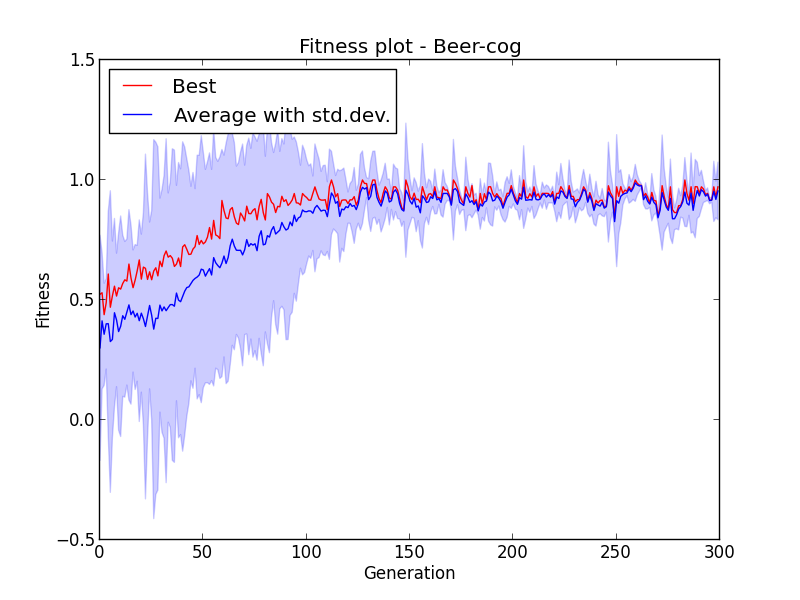
\includegraphics[width=1.0\textwidth]{mincog_fitness}}
\paragraph{}We ran the test three times. The first time, we got an agent that tried to catch everything. The second time, we got one with an interesting, but inconsistent, avoidance strategy. The last one worked almost perfectly, and an expanded description follows here:
\paragraph{}To begin with, the tracker moves right at a speed of two units per turn. It keeps doing this until it sees an object, at which point it slows down to determine the size. If it's a small object, it stops and catches it. If it's a large object, it speeds up and then stops to the right of the object. It will never move left, but two units per turn gives plenty of time to wrap around and reach an object directly to the left, and get out of harm's way if necessary.

\section{Changed scenario}
\paragraph{}We decided to change the direction of the falling objects to se if this had any effect on the evolution of the agent. Instead of having the object fall straight down it now moves diagonally to the right, moving one unit horizontally for each unit dropped downwards.
\paragraph{}Naturally this changed the solutions generated by the algorithm, as the problem is no longer the same, but the success rate was not changed noteworthy. Evolution came up with three main ways to solve this, described in order of most commonly occurring to least commonly occurring:
\begin{itemize}
\item{The agent moves slowly to the left, looking for an object. When it finds an object it examines it, and then follows it back to the right if it is an object it is supposed to catch. The most common solution to dodging is to just keep moving to the left, sometimes with increased speed. Another more rare dodging mechanic was to stop as it saw a large object, or slightly after, making sure it wouldn't catch the object after having moved enough to get under it again.}
\item{The agent moves at high speed to the right, trying to catch up with the falling objects. When it finds an object it slows down to examine it. If the item is small enough it keeps moving at the reduced speed, but if the item is large, and the agent has evolved the ability to dodge, it usually increases the speed again to outrun the falling object. Evolving the ability to dodge was somewhat rarer in this case.}
\item{The last movement scheme is to just stand still till an object appears above the agent. If the object is small enough it will start following it, while if the object is large it will try to dodge it. The most common way of dodging is to just stand still, but on some attempts it evolves the ability to move fast to the left to a safe spot before stopping again.}
\end{itemize}
\paragraph{}While evolving solutions to the case where the object falls with a horizontal speed we realised that the problem is not much harder than the original problem of the object falling straight down. If we take a solution to the original problem and manually add the speed of the falling object to the agent we have a fully working solution. This means that the logic is the same, and the network just has to evolve to a different base speed.

\section{Changed CTRNN topology}
\paragraph{}In an attempt to make the solutions smarter we tried to increase the number of hidden nodes in the CTRNN. The number of hidden nodes was set to 4. This would lead to more internal connections, something we thought would give it a more sophisticated memory, and thus increase the ability to remember that it had encountered large objects.
\paragraph{}Sadly this was not the case. The general form of the good solutions remained much the same as in the case where we had two hidden nodes; it tracked sideways looking for objects to catch, then stopped if it found a smaller object. The most common strategy to dodge objects found was to simply keep moving and hoping it would not hit, sometimes with increased speed for a short time.
\paragraph{}The most notable difference compared to the unmodified case is that the agent seems to search for falling objects at a higher speed. This is most likely due to the fact that the output nodes have more incoming edges, allowing for higher values in either direction.
\subsection{Conclusion}
\paragraph{}While the modification did not prove to evolve more intelligent agents (stopping in a safe spot after having observed a larger object) like we hoped, it still did a good job of solving the problem given. In hindsight it was unreasonable to hope for such an improvement without modifying the fitness function to reward such a behaviour, coupled with the fact that continous movement is a sound dodging strategy in an environment where such a strategy has a rather small chance to hit an object.

\section{Changed Parameter Ranges}
\paragraph{}While testing, we found that most of the evolved agents would search at a speed of one unit per turn. This would often turn out to be too slow, so we decided to see if we could encourage faster movement by changing some parameter. Allowing weights to span [-10.0, +10.0] (as opposed to [-5.0, +5.0]) seemed like a natural choice for this. We ran the tests with population size 75, litter size 75, and generation count 200.
\subsection{Results}
\paragraph{}We did five runs, and these were the results:
\begin{enumerate}
\item{Searches with speed 4. Slows down to check size. Fails to catch size 4 objects.}
\item{Starts at speed 4, then slows down to 3. Doesn't catch anything while running at speed 4. Fails to catch size 4 objects.}
\item{Searches at speed 4, catches all small objects. Avoidance: Sometimes gets out of the way and continues at speed 1, other times gets out of the way and then continues at oscillating speed.}
\item{Search speed oscillates with a 4-4-0 pattern. If it gets lucky and stops under a small object, it stays there to catch it, otherwise it just keeps going}
\item{Searches at speed 4. Catches most of the time, sometimes runs past and then catches on the second run. Avoidance: Slows down for a bit, then goes back to speed 4.}
\end{enumerate}
\paragraph{}We clearly see that we accomplished what we set out to do, which was to increase the search speed. However, this introduces new problems, such as catching not always working properly. A search speed of 2 or 3 seems to work best, so maybe the [-10.0, 10.0] range was a bit much.

\section{Multiple-Objective Evolutionary Algorithm}
\subsection{Methodology}
\paragraph{}We chose to implement the NSGA-II algorithm, as described in the lecture slides and the original paper by Deb et.al. To avoid multiple inclusion of individuals with identical fitness in all parameters, we had to add the rule that older individuals dominate newer ones, all other things being equal. The fitness parameters used were normalized score and total movement, as suggested in the problem text.
\paragraph{}Since we were looking for several solutions rather than just one, we bumped up the population size to 500, and ran for 200 generations in order to get a good result.

\subsection{Results}
\paragraph{}

\section{Works Cited}
\begin{itemize}
\item{IT3708 lecture slides}
\item{K. Deb, A. Pratap, S. Agarwal and T. Meyarivan ``A Fast and Elitist Multiobjective Genetic Algorithm: NSGA-II'' \textit{IEEE Transactions on Evolutionary Computation}, Vol. 6, No. 2, pp. 182-197, Apr. 2002}
\end{itemize}

\end{document}
